Após desenvolver os métodos descritos nas seções \ref{sec:descida_max}, \ref{sec:grad_conj}, \ref{sec:netwon}, \ref{sec:newton_mod} e \ref{sec:quase_newton} como funções do MATLAB, foi implementada uma interface gráfica, tornando a utilização desses métodos mais amigável ao usuário.\\

\par Assim como no primeiro Trabalho, essa interface foi desenvolvida no próprio MATLAB, em um ambiente chamado \textit{GUIDE} (Graphical User Interface Development Environment) que permite a criação da janela do programa com poucos cliques, conforme ilustrado na figura \ref{fig:guide}. A programação dos elementos da interface é feita em um arquivo *.m que está ligado a interface gráfica, armazenada em uma figura do matlab (*.fig).

\begin{figure}[H]
	\begin{center}
		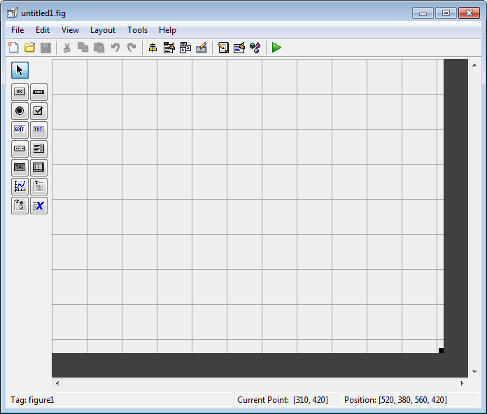
\includegraphics[width=10cm]{GUIDE}   
		\caption{Ambiente de desenvolvimento de interface gráfica \textit{GUIDE}.}
		\label{fig:guide}
	\end{center}
\end{figure}

O programa desenvolvido foi denominado \textbf{Busca de Mínimos Iterativa} e pode ser visto sua janela inicial na figura \ref{fig:gui}.

\begin{figure}[H]
	\begin{center}
		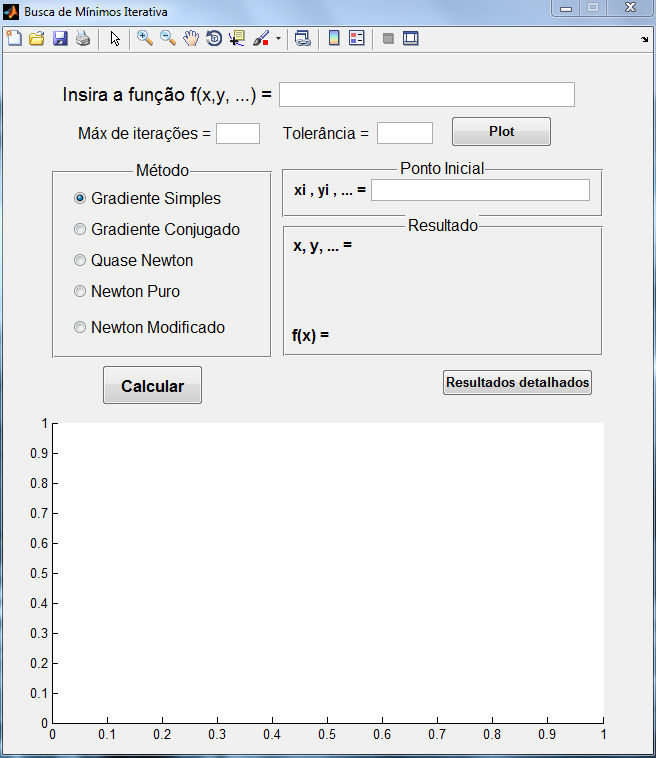
\includegraphics[width=10cm]{GUI}   
		\caption{Janela do programa de Busca de Mínimos Iterativa.}
		\label{fig:gui}
	\end{center}
\end{figure}

\par O usuário começa colocando a expressão da função que ele deseja minimizar, lembrando de pontuar as multiplicações com um asterisco (*). Deve se definir então, \textbf{o método} a ser utilizado; o \textbf{máximo de iterações}, para que o programa não rode indefinidamente em casos em que não haja convergência; a \textbf{tolerância} desejada para o resultado procurado; e o \textbf{ponto inicial} de onde o método irá partir. É possível, com o botão de \textbf{plot}, verficar a forma da função (caso seja de 2 variáveis) antes de rodar a busca, assim podemos verificar se a função atende às especificações sem ter que esperar o programa rodar e ficar procurando um mínimo, quando a função pode não apresentar um. \\

\par Feito isso, basta clicar no botão \textbf{Calcular} e os resultados serão exibidos ao lado, o valor de x que dá o mínimo da função e o valor minímo nesse ponto. Além disso, para funções de 2 variáveis também é exibido o \textbf{gráfico da função} dentro do intervalo pedido, o mínimo é destacado com um círculo vermelho e o ponto inicial com um círculo branco. Vale ressaltar que o programa encontra mínimos para funções de n variáveis, $\forall n \varepsilon \mathds{N}$.   \\
